% xelatex
\documentclass[letterpaper,
		%twocolumn,
		10pt]{article}
\usepackage[utf8]{inputenc}
\usepackage{metalogo}
\usepackage{xifthen}
\usepackage[colorlinks=true,urlcolor=Blue]{hyperref}
\usepackage{graphicx}
\usepackage{fontspec}
\usepackage[T1]{fontenc}
\usepackage[dvipsnames]{xcolor}
\usepackage{titlesec}
\usepackage[margin=1in]{geometry}
\usepackage{titling}
\newfontfamily\cfont{Noto Sans CJK SC}
\usepackage{libertine}
\usepackage{ctex}

% Macro to allow image links in XeLaTeX
\ifxetex
  \usepackage{letltxmacro}
  \setlength{\XeTeXLinkMargin}{1pt}
  \LetLtxMacro\SavedIncludeGraphics\includegraphics
  \def\includegraphics#1#{% #1 catches optional stuff (star/opt. arg.)
    \IncludeGraphicsAux{#1}%
  }%
  \newcommand*{\IncludeGraphicsAux}[2]{%
    \XeTeXLinkBox{%
      \SavedIncludeGraphics#1{#2}%
    }%
  }%
\fi
%%%%%%%

% Bold contents of a link
\let\oldhref\href
\renewcommand{\href}[3][blue]{\oldhref{#2}{\color{#1}{#3}}}

% Your name goes here:
\author{庄宇林}

% Update date set to last compile:
\date{\today}

% Custom title command.
\renewcommand{\maketitle} {
    \begin{minipage}[t]{.5\textwidth}
        {\Huge \bfseries{\theauthor}}
        % \par \phone{} 18650395493
        % \par \email{} :     & \href{mailto:307256078@qq.com}{307256078@qq.com}\\
        % \vfill
        \begin{tabular}{rp{.75\linewidth}}
            \baselineskip=20pt
            \phone{} :     & \href{tel:18650395493}{+18650395493}\\
            \email{} :     & \href{mailto:307256078@qq.com}{307256078@qq.com}
            % \www{} : &\href{https://www.lukesmith.xyz}{https://lukesmith.xyz}
        \end{tabular}
        {\footnotesize\color{gray} (Last updated \thedate.)}
	\end{minipage}

    \hfill\footnotesize
    \begin{minipage}[b]{.25\textwidth} % {
        \smash{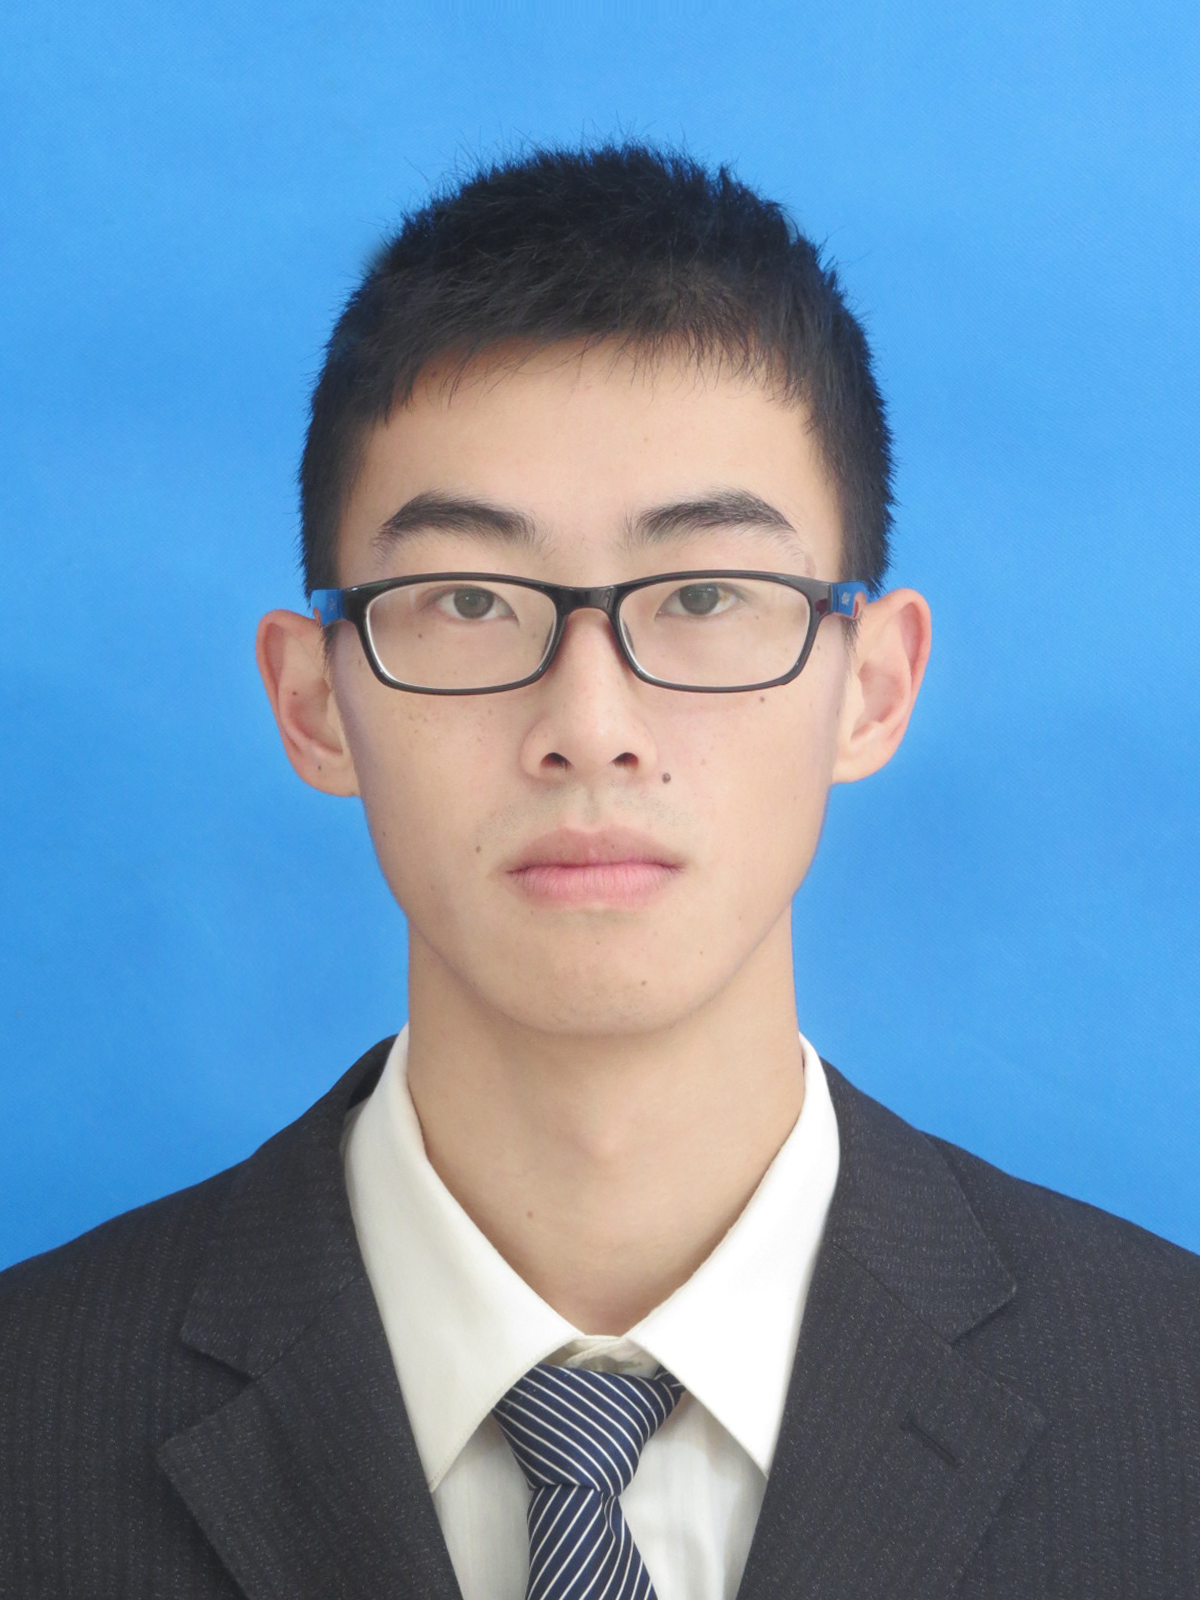
\includegraphics[height=1.5in]{cv/head.jpg}}
	\end{minipage}
}

% Setting the font I want:
\renewcommand{\familydefault}{\sfdefault}
\usepackage{sqrcaps}

% Making the \entry command
\newcommand{\entry}[4]{
\ifthenelse{\isempty{#3}}
{\slimentry{#1}{#2}}{

\begin{minipage}[t]{.15\linewidth}
\hfill \textsc{#1}
\end{minipage}
\hfill\vline\hfill
\begin{minipage}[t]{.80\linewidth}
{\bf#2}\\\textit{#3} \footnotesize{#4}
\end{minipage}\\
\vspace{.2cm}
}}

\newcommand{\slimentry}[2]{

\begin{minipage}[t]{.15\linewidth}
\hfill \textsc{#1}
\end{minipage}
\hfill\vline\hfill
\begin{minipage}[t]{.80\linewidth}
#2
\end{minipage}\\
\vspace{.25cm}
}% end \entry command definition

% Some macros because I'm lazy:
\newcommand{\uga}{University of Georgia}
\newcommand{\gsu}{Georgia State University}
\newcommand{\ua}{University of Arizona}

% Macros for people's names including link to their websites
\newcommand{\tgb}{\href{http://coglanglab.com}{Tom Bever}}
\newcommand{\mas}{\href{http://dingo.sbs.arizona.edu/~massimo/}{Massimo Piattelli-Palmarini}}
\newcommand{\rob}{\href{https://rhenderson.net/}{Robert Henderson}}
\newcommand{\mike}{\href{http://www.u.arizona.edu/~hammond/}{Mike Hammond}}
\newcommand{\simin}{\href{http://www.u.arizona.edu/~karimi/}{Simin Karimi}}
\newcommand{\heidi}{\href{http://heidiharley.com/}{Heidi Harley}}
\newcommand{\amy}{\href{https://linguistics.arizona.edu/user/amy-fountain}{Amy Fountain}}
\newcommand{\vera}{\href{https://www.gsstudies.uga.edu/people/vera-lee-schoenfeld}{Vera Lee-Schoenfeld}}
\newcommand{\tim}{\href{http://www.rom.uga.edu/directory/timothy-gupton}{Tim Gupton}}
\newcommand{\pilar}{\href{http://www.rom.uga.edu/directory/pilar-chamorro}{Pilar Chamorro}}
\newcommand{\jenni}{\href{https://www.jennimariapalomaki.com/}{Jennimaria Palomäki}}

\let\lineheight\baselineskip

% Link images
\newcommand{\pdf}{
\includegraphics[height=.85em]{cv/pdf.png}}
\newcommand{\yt}{
\includegraphics[height=.85em]{cv/yt.png}}
\newcommand{\gh}{
\includegraphics[height=.85em]{cv/gh.png}}
\newcommand{\www}{
\includegraphics[height=.85em]{cv/www.png}}
\newcommand{\email}{
\includegraphics[height=.85em]{cv/email.png}}
\newcommand{\phone}{
\includegraphics[height=.85em]{cv/phone.png}}
\newcommand{\ruijie}{
\includegraphics[height=.85em]{cv/ruijie.png}}
\newcommand{\fzu}{
\includegraphics[height=.85em]{cv/fzu.png}}

% Custom section spacing and formatting
\titleformat{\part}{\Huge\scshape\filcenter}{}{1em}{}
\titleformat{\section}{\Large\bf\raggedright}{}{1em}{}[{\titlerule[2pt]}]
\titlespacing{\section}{0pt}{3pt}{7pt}
\titleformat{\subsection}{\large\bfseries\centering}{}{0em}{\underline}%[\rule{3cm}{.2pt}]
\titlespacing{\subsection}{0pt}{7pt}{7pt}

% No indentation
\setlength{\parindent}{0in}

\begin{document}
% hhaha
\maketitle

\section{基本信息}

\begin{minipage}[t]{.5\linewidth}
    \begin{tabular}{rp{.75\linewidth}}
        \baselineskip=20pt
        \email{} :     & \href{mailto:307256078@qq.com}{307256078@qq.com}\\
        \www{} : &\href{https://www.lukesmith.xyz}{https://lukesmith.xyz}
    \end{tabular}
\end{minipage}
\begin{minipage}[t]{.5\linewidth}
    \begin{tabular}{rl}
        \gh{} : & \href{http://github.com/LukeSmithxyz}{github.com/LukeSmithxyz}\\
        \yt{} : &\href{http://youtube.com/c/LukeSmithxyz}{youtube.com/c/LukeSmithxyz}
    \end{tabular}
\end{minipage}

\begin{itemize}
\item Maintainer and developer of an Arch Linux-based metadistribution at \href{https://larbs.xyz}{https://larbs.xyz \www}.
\item Doctoral student in linguistics at the \href{https://linguistics.arizona.edu}{University of Arizona \www}, focusing mostly on deriving linguistic traits and tendencies from non-linguistic externals and theoretical reform.

For more information, go here: \href{https://lukesmith.xyz/linguistics}{https://lukesmith.xyz/linguistics \www}.
\item Since late 2016, I run a \href{https://youtube.com/c/lukesmithxyz}{YouTube channel \yt} mostly on technology tutorials and Linux configuration and system management.
\end{itemize}

\section{教育经历}

\entry{2016--2019}
	{硕士, Fuzhou University (\href{https://www.fzu.edu.cn}{福州大学\fzu})}
	{fuzhou, China}
	{控制理论与控制工程 Major in Syntax; minor in \textbf{Romance Languages}. Thesis: \textit{External Possession and the Undisentanglability of Syntax and Semantics} \href{https://lukesmith.xyz/thesis.pdf}{\pdf}. Advisor: \vera.}

\entry{2012--2016}
    {本科, Fuzhou University (\href{https://www.fzu.edu.cn}{福州大学\fzu})}
	{福州fuzhou, China}
	{电气工程与自动化专业}

\entry{2009--2012}
	{B.A. in International Economics and Modern Languages}
	{Andrew Young School of Policy Studies, \gsu, Atlanta}
	{Specializations in Spanish and Chinese. Certificates in Economic History and International Trade.}

\section{工作经历}

\entry{2019--now}
    {Software Engineer (\href{https://www.ruijie.com.cn}{锐捷网络\ruijie})}
	{fuzhou, China}
	{Focusing on bsp ethernet driver}

\section{工作内容}

More teaching information, along with my \textbf{teaching evaluations} and some materials can be found on my website at \href{http://www.lukesmith.xyz/classes}{lukesmith.xyz/classes \www}.

%\entry{2017--Now}{``Historical Linguistics''}{YouTube}{An ongoing lecture series on YouTube, originally focusing on Historical Linguistics and Linguistic Thought, but branching out to more general topics.}

\entry{2018}
	{LING150 -- ``Language'' Online Class}
	{\ua}
	{With \amy.}

\entry{2017--2018}
	{ESOC210 -- ``The History of Hacking and Open Source Culture'' -- Graduate Assistant}
	{\ua}
	{Under David Seng. Grader.}

\entry{2016}
	{LING300 -- ``Introduction to Syntax'' -- Teaching Assistant}
	{\ua}
	{Under \simin. Helped introduce undergraduates to the Gospel of Chomsky. Served as a substitute for main professor when gone, graded work and did administrivia.}

\entry{2015--2017}
	{LING150 -- ``Language'' -- Teaching Assistant}
	{\ua}
	{With \amy. I teach Friday sessions and conduct recitations for a break-out section of an auditorium classroom. I conduct my own activities and lectures off of my own syllabus.}

\entry{2014--2015}
	{LING2100 -- ``Study of Language'' -- Instructor \href{https://lukesmith.xyz/dox/2100/2100_fa.pdf}{\pdf} \href{https://lukesmith.xyz/dox/2100/2100_sp.pdf}{\pdf}}
	{\uga}
	{I worked through my own syllabus and class plan and focus mainly on how language relates to wider issues in cognitive science. Also focused on the philosophy of language and historical linguistics.}

\entry{2014}
	{LING3150 -- ``Generative Syntax'' -- Co-teacher}
	{\uga}
	{Covered Phrase-Structure Rules and X-bar Theory. A writing intensive course. Taught with \jenni.}

\entry{2014}
	{Writing Intensive Program -- Teaching Assistant}
	{\uga}
	{Guided and graded essay-writing for linguistics students.}

\section{Presentations}

Current projects and other information can be found on \href{https://lukesmith.xyz/linguistics.html}{https://lukesmith.xyz/linguistics \www}.

\entry{Soon}
	{``The Evolution of the Ibero-Romance Irregular Imperfect: A Constraint-based Analysis''}
	{28th Annual Symposium on Hispanic and Luso-Brazilian Literature, Language and Culture}

\entry{2017}
	{``Scope without Syntax: Towards a Game Theoretic Approach'' \href{https://lukesmith.xyz/dox/ling/luke_synsalon.pdf}{\pdf}}
	{\ua{} Synsalon}

\entry{2017}
	{``Language as Synesthesia'' \href{https://www.youtube.com/watch?v=he4-K3Ir1PY&list=PL-p5XmQHB_JQdpstJQ4DH18GZ8qt3KVxq}{\yt} \href{https://lukesmith.xyz/dox/etc/luke_synesthesia.pdf}{\pdf}}
	{Seminar on language and consciousness}
	{Clarification of some points from \href{https://www.youtube.com/watch?v=fEY5qkgH3fo&list=PL-p5XmQHB_JQdpstJQ4DH18GZ8qt3KVxq&index=1}{my qualifying paper.}}

\entry{2015}{``Towards Biolinguistic Clarity in Generative Syntax'' \href{https://www.youtube.com/watch?v=yk03pXPGiVs}{\yt}}{The Interdisciplinary Linguistics Conference at UGA, 2015}

\entry{2015}
	{``Syntax is for Real! -- Parameterization of Head Movement in Korean and its Effects on Scope and Alternations''}
	{LSUGA Tiny Talks}

\entry{2015}
	{``External Possession and the Undisentanglability of Syntax and Semantics''}
	{\uga\ Linguistics Program Spring Colloquium}

\entry{2013}
	{``The acquisition of \emph{tú} and \emph{usted} by English speakers: A study of non-native knowledge and usage of forms of address''}
	{Georgia State Undergraduate Research Conference}

\entry{2012}
	{``Theories of contraction: A survey of macroeconomic theories of depression''}
	{Georgia State Undergraduate Research Conference}

\section{Guest Lectures}

\entry{Soon}
	{Linguistics Isn't 60 Years Old!}
	{Guest Lecture}
	{For \simin's class \textit{Major Works in Syntax}}

\entry{Soon}
	{Quantifier Scope is Just All Fun and Games!}
	{Linguistics Department Graduate Student Showcase}
	{}

\entry{2017}
	{``The Origins and Mechanics of the Greek Alphabet'' \href{https://lukesmith.xyz/dox/etc/greek_alphabet.pdf} {\pdf}}
	{Guest Lecture}
	{For Shannon Grippando's class \textit{The Psychology of Writing Systems}}

\entry{2016}
	{``The Phonetics of Language''}
	{Guest Lecture}
	{For Amy Fountain's class \textit{Language}}

\entry{2016}
	{``Constituent Structure---What is it and where does it come from?''}
	{Guest Lecture (series of 3)}
	{For \simin's class \textit{Introduction to Syntax}}

\entry{2016}{``An Introduction to Minimalism''
	\href{https://lukesmith.xyz/dox/etc/luke_doug_min.pdf}{\pdf}
	\& ``Optimizing Structure''
	\href{https://lukesmith.xyz/dox/etc/luke_doug_allphon.pdf}{\pdf}
	}{Guest Lectures}{For Doug Merchant's class \textit{Generative Syntax}}


\entry{2015}{``Syntactic Theory and Psycholinguistics''
	\href{https://lukesmith.xyz/dox/etc/syn_psycho.pdf}{\pdf}
	}{Guest lecture}{For Doug Merchant's class \textit{Psychology of Language}}

\section{Languages}

\entry{Human}
	{Spanish, Mandarin, Latin, some Persian and French, reading knowledge of classical Greek and most Romance languages. Grammatical knowledge of a many Indo-European languages, Korean and others.}
	{}
	{}

\entry{Machine}
	{Python, Perl, R, PHP, Matlab/GNU Octave, bash/shell, some superficial knowledge of C, common LISP and Haskell; markup languages including {\LaTeX}/{\XeTeX}, R Markdown, HTML, CSS.}
	{}
	{}

\section{Tools I Use}

I have lots of tutorials on many of these programs and tools on my \href{https://youtube.com/c/lukesmithxyz}{my YouTube channel \yt}.

\subsection{Usual Workflow}

I use a \textbf{vim}-based setup in a tiling window manager (\textbf{i3-gaps}). I compile documents using \textbf{R Markdown} or \textbf{\LaTeX}, and \textbf{biber} for references. I prefer to do multimedia manipulation in the terminal with tools like \textbf{imagemagick} and \textbf{ffmpeg} for extensibility's sake.
I've run Microsoft, MacOS and GNU/Linux systems (both Debian and Arch-based varieties, as well as Void Linux).

\subsection{Programs I'm Familiar With}

tmux, ssh, RStudio, Blender (mostly for video-editing), Praat, Audacity, E-Prime, GIMP, pandoc, Jupyter. I've managed websites manually via ssh and vim using HTML/CSS/PHP and with tools such as Github Pages (Jekyll) WordPress via either cpanel or wp-cli. Some experience with myBB.

\section{Public Code and Scripts}

\entry{2018}
	{mutt and offlineIMAP wizard \href{https://github.com/lukesmithxyz/mutt-wizard}{\gh}}
	{A fully-featured configuration tool.}
	{A tool for automatically configuring mutt, offlineIMAP, notmuch and other parts of a full email system with automatic detection of IMAP and SMTP protocols and automatic password encryption}

\entry{2017--2018}
	{shortcut-sync \href{https://github.com/lukesmithxyz/shortcut-sync}{\gh}}
	{A small system for synchronizing configs between bash and other shells, ranger and qutebrowser.
	}
	{}

\entry{In Progress}
	{Corpus Latinum Lucæ \href{https://github.com/LukeSmithxyz/corpus-latinum}{\gh}}
	{A planned linguistic corpus of the Latin language, to be searchable by regexes and grammatical category, with an interface written in Python.}
	{As of now I've constructed the parser to generate the corpus from raw text files.}

\entry{2017--Now}
	{Luke's Auto-Rice Bootstrapping Scripts (LARBS) \href{https://larbs.xyz}{\www} \href{https://github.com/LukeSmithxyz/larbs}{\gh}}
	{A dynamic installer for an i3wm Arch Linux distribution}
	{}

\entry{2016--Now}
	{Voidrice \href{https://github.com/LukeSmithxyz/voidrice}{\gh}}
	{Linux dotfiles}
	{A set of GNU/Linux dotfiles that I popularized on YouTube, aiming at creating a powerful, optimized, all-purpose and lightweight general computing environment. Innovated dynammically configured and synced rc files.}

\entry{2015}
	{http://LukeSmith.xyz \href{http://LukeSmith.xyz}{\www}}
	{My website}
	{Written from scratch. Modern traditional feel. I generate the website offline with PHP and upload a static version of only HTML/CSS.}

\entry{2016--2017}
	{/Comfy/ Arch}
	{Automatic ricing tool}
	{A web-based deployment system for configuration files which focuses on enabling novice Linux users to get immersed quickly in advanced ricing environments. No longer actively maintained as it has been largely replaced by LARBS (above).}

\entry{2013}
	{Vulgarizer}
	{Sound Change Simulator}
	{A string-manipulation paradigm written in Python for simulating phonetic and phonological change over time. The original implementation focused on modeling changes between Latin and Spanish and then other Romance languages, but if I continue the project, my hope is to generalize this.}

%\subsection{Other}

%My build of the the suckless \href{https://github.com/LukeSmithxyz/st}{simple terminal (st) \gh} with added homerow binds and small improvements.

\section{Online Tutorials}

I produce screencasts and produce other videos for public use as tutorials on YouTube on my channel. \href{https://youtube.com/c/LukeSmithxyz}{\yt}
As of January 2018, over 13,000 subscribers, with 1.4 millions views on over 100 different videos. All of these series below are ongoing.

\entry{R / Statistics \href{https://www.youtube.com/playlist?list=PL-p5XmQHB_JQlsPHtcxNWpvDudyoWB2kH}{\yt}}
	{\footnotesize
	\href{https://www.youtube.com/watch?v=WlCWQrKQQI4}{[1]: Arithmetic, Variables and Vectors},
	\href{https://www.youtube.com/watch?v=pgRvPNo6HaY}{[2]: Basic Statistical Functions and Logic},
	\href{https://www.youtube.com/watch?v=DDzVtu24dbk}{[3]: Dataframes, Subsetting and Ifelse}
	}
	{}{}

\entry{{\LaTeX}
	\href{https://www.youtube.com/playlist?list=PL-p5XmQHB_JSQvW8_mhBdcwEyxdVX0c1T}{\yt}}
	{\footnotesize
\href{https://youtube.com/watch?v=NwnYHoNtfJ0}{[0]: Installation}
\href{https://youtube.com/watch?v=mfRmmZ_84Mw}{[1]: Compiling, Titles, Sections, Formatting, Syntax}
\href{https://youtube.com/watch?v=25LExaNtdF0}{[2]: Labels, References and Lists}
\href{https://youtube.com/watch?v=46piog3Fzp4}{[3]: Bibliographies}
\href{https://youtube.com/watch?v=VjsX4tznW40}{[4]: Résumé-making Part 1}
\href{https://youtube.com/watch?v=o5-BZ7JmYWk}{[5]: Résumé-making Part 2}
\href{https://youtube.com/watch?v=zgThRPjy-vw}{[6]: Images, Figures}
\href{https://youtube.com/watch?v=zEjBCQhND2c}{[7]: Beamer Slideshow Presentations}
\href{https://youtube.com/watch?v=rvgP7IMeUn8}{[8]: Macros}
}
{}{}

\entry{vim
	\href{https://www.youtube.com/playlist?list=PL-p5XmQHB_JSTaEPygu1DZjuFfb704Uv7}{\yt}
	}
	{\footnotesize
\href{https://youtube.com/watch?v=wRFEBw02aT8}{Macros}---
\href{https://youtube.com/watch?v=yNOkCYuPt3E}{Workflow with LaTeX}---
\href{https://youtube.com/watch?v=jUfw7aHD_xY}{Basic Tips After Vimtutor}---
\href{https://youtube.com/watch?v=K_8_gazN7h0}{SC-IM - Vim-based Terminal Spreadsheet Editor}---
\href{https://youtube.com/watch?v=Q4I_Ft-VLAg}{Custom code snippets, for IDE functionality}---
\href{https://youtube.com/watch?v=GqoJQft5R2E}{Vi-mode in bash}---
\href{https://youtube.com/watch?v=ez1XBUqbS68}{Spell-checking and Dictionaries}---
\href{https://youtube.com/watch?v=NzD2UdQl5Gc}{How vim Makes my Daily Life Easier}
}{}{}

\entry{Linux}
	{Videos on hacking and modifying Linux graphical environments particularly on i3-gaps, including customization, window management, program-shortcutting, optimization.
	\href{https://www.youtube.com/playlist?list=PL-p5XmQHB_JTcMSvPmXMzNe7ZPMxEx_Oz}{\yt}}
	{}
	{}

\section{Service}
\entry{Soon}
	{Coyote Papers Editor for the 2018 Arizona Linguistics Circle}
	{\ua}
	{}

\entry{2017--Now}
	{Manager for Tom Bever's Language and Cognition Lab site \href{http://coglanglab.com}{\www}}
	{\ua}
	{\href{http://coglanglab.com}{http://coglanglab.com}}

\entry{2017}
	{Arizona Linguistic Circle Peer-Reviewer}
	{\ua}
	{Judged and gave feedback for scholarly articled submitted for the Arizona Linguistics Circle.}

\entry{2015--2016}
	{Indo-European Reading Group Director}
	{\ua}
	{Covering general historical linguistics, and the particulars of PIE morphology, phonology and development. Group materials located at \href{http://www.lukesmith.xyz/pie}{lukesmith.xyz/pie \www}.}

\entry{2014--2016}
	{LSUGA Website Manager}
	{\uga}
	{Created and managed the LSUGA website, \href{http://www.lsuga.com}{http://www.lsuga.com}. (Now apparently reformatted.)}

\entry{2014--2015}
	{LSUGA Interdisciplinary Conference in Linguistics Committee Member}
	{\uga}
	{Managed email, reviewed papers and did audio and video for conference.}

\entry{2014--2015}
	{Graduate Student Mentor}
	{\uga}
	{}

\entry{2014}
	{Socio-Paths Sociolinguistics Reading Group Co-director}
	{\uga}

\entry{2014}
	{Typology Reading Group Director}
	{\uga}
	{Covered classical Greenbergian typology, particularly with relevance to historical linguistics.}


\section{Writings}

Section incomplete. Only contains major degree requirements now. To be updated. More minor squibs of mine can be found at \href{https://lukesmith.xyz/linguistics}{https://lukesmith.xyz/linguistics \www}.

\entry{SOON}
	{Unnamed dissertation}
	{Dissertation, \ua}
	{
	Probable committee?: \tgb, \mike, \mas, \rob.
	}

\entry{2017}
{Scope Without Syntax: A Game Theoretic Approach
	\href{https://lukesmith.xyz/qp2.pdf}{\pdf}
	\href{https://github.com/LukeSmithxyz/scope-without-syntax}{\gh}
	}
	{Second qualifying paper, \ua}{
	Committee: \rob, \mas, \tgb, \mike.
	}

\entry{2017}
	{Syntax Without Syntax
	\href{https://lukesmith.xyz/qp1.pdf}{\pdf}
	\href{https://www.youtube.com/watch?v=fEY5qkgH3fo}{\yt}
	\href{https://github.com/lukesmithxyz/syntax-without-syntax}{\gh}
	}{First qualifying paper, \ua}{
	Committee: \mike, \simin, \heidi.
	}

\entry{2015}
	{External Possession and the Undisentanglability of Syntax and Semantics \href{https://lukesmith.xyz/thesis.pdf}{\pdf}}
	{Master's thesis, \uga}{
	Committee: \vera, \tim, \pilar.
	}

\section{Hobbies}

Classical languages, human evolution and prehistory, free (i.e. libre) software, survivalism, cybernetics, medieval thought, Rhaeto-Romance poetry. I run a web forum at \href{https://forum.lukesmith.xyz}{forum.lukesmith.xyz}.

\section{References}

\begin{itemize}
	\item Email me \href{mailto:luke@lukesmith.xyz}{\email} with your interests in me and I'll refer you to someone who can vouch for me or defame me, depending on what you want.

\item I upload all of my teaching evaluations to \href{https://lukesmith.xyz/classes\#evals}{https://lukesmith.xyz/classes\#evals \www} and they can be read there.
\end{itemize}


\end{document}
